%!TEX root = ../dokumentation.tex

\chapter{Training und Evaluation eines Klassifikationsmodells} \label{ch:crispDm_2}

\section{Training von Modellen} \label{sec:modeling}

% TODO: Review and add ideas for modeling

\begin{itemize}
    \item Datenquellen erst einzeln trainieren
    \item Datenquellen in verschiedenen Kombinationen trainieren
    \item Undersampling nach Partei 
\end{itemize}

\subsection{Feature Engineering} \label{subsec:featureEngineering}

% TODO: This are only ideas and options for additional features 
% TODO: Evaluate the features

\subsubsection{Sentiment}

Eine Limitation von den herkömmlichen \ac{ML} Modellen ist die Klassifikation von Polysemie \autocite[48\psq]{kowsari_text_2019}. 

% TODO: Find source

Ein Ansatz, um diese Limitation zu mindern, ist es, den Sentiment eines Textes zu berechnen. Ziel dieser Technik ist es nicht nur festzustellen, ob sich ein Politiker zum Beispiel zur \ac{AfD} äußert oder nicht, sondern ebenfalls, ob seine Äußerungen positiv, neutral oder negativ sind.

% TODO: Add timeline for ML Models

Die einfachste Methode, um den Sentiment von deutschen Texten zu ermitteln, sind Sentiment-Wörterbücher wie \textit{SentiWS}, \textit{BAWL-R} und \textit{GermanPolarityClues} \autocite[1627\psq]{guhr_training_2020}. CNN, SVM, Bi-LSTM, \dots

Die bisherigen regelbasierten Ansätze, als auch \ac{ML} Modelle wie \acp{SVM}, \acp{CNN} und \acp{LSTM} erreichen einen F1-Score von bis zu \num{74.9}. Alternativ zu diesen Ansätzen stellen \textcite{guhr_training_2020} ein \ac{BERT}-basiertes \ac{ML} Modell bereit. Dieses wurde mittels der folgenden Datensätze trainiert: \textit{PotTS}, \textit{SB10k}, \textit{GermEval-2017}, \textit{Scare}, \textit{Filmstarts}, \textit{holidaycheck}, \textit{leipzig-wikipedia} und \textit{Emotions}. Das Modell erreicht einen F1-Score von \num{0.9636} und ist somit den vorherigen Modellen deutlich überlegen \autocite[1631]{guhr_training_2020}.

\subsubsection{Gendern}

- Verhältnis Wörter/Gendersterne oder True/False
- Check mit RegEx ob gegendert wird und setze variable

\subsubsection{Dokumenttyp}

- Tweet, Speech, \dots

\subsection{Baseline Models}

% TODO: Update scores

\begin{table}[H]
    \centering
    {\footnotesize
    \begin{tblr}{width=\textwidth, hlines, vlines}
        \textbf{Modell} & \textbf{Datensatz} & \textbf{Precision} & \textbf{Recall} & \textbf{\(F_1\) Score} \\ 

        \textbf{SVM + \acs{BoW}} & Tweets & \num{0.59} & \num{0.59} & \num{0.59} \\
        \textbf{SVM + \acs{BoW}} & Wahlpro\-gramme & \num{0} & \num{0} & \num{0} \\
        \textbf{SVM + \acs{BoW}} & Reden & \num{0} & \num{0} & \num{0} \\

        \textbf{Kombiniert} & \textbf{\num{0}} & \textbf{\num{0}} & \textbf{\num{0}} \\
    \end{tblr}
    }
    \caption{Scores für Baseline Modelle auf Basis von \acs{BoW} und \acs{TF-IDF}} \label{tab:overviewScoresBaseline}
\end{table}

\subsection{Advanced Models}

\subsubsection*{FastText}

% TODO: Update and add plots for other datasets

\begin{figure}[H]
    \begin{subfigure}{.5\textwidth}
      \centering
      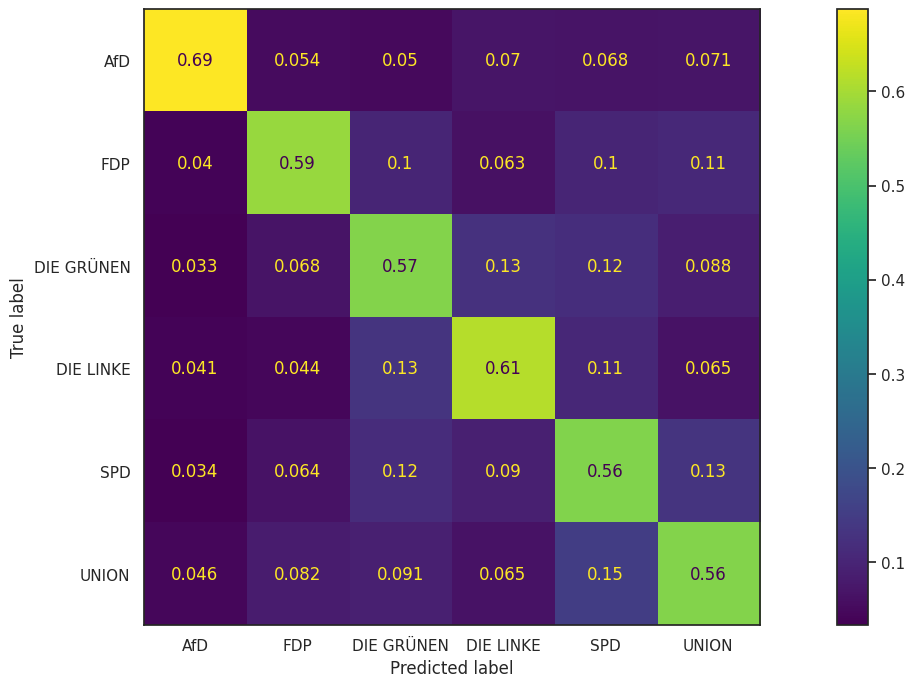
\includegraphics[width=0.9\linewidth]{data/images/tweets/fasttext_tweets_confusion.png}
      \caption{Tweets von \acs{MdB}} \label{sfig:confusionMatrixFastTextTweets}
    \end{subfigure}
    \begin{subfigure}{.5\textwidth}
      \centering
      \missingfigure{Wahlprogramme}
      \caption{Wahlprogramme} \label{sfig:confusionMatrixFastTextManifest}
    \end{subfigure}
    \begin{subfigure}{.5\textwidth}
      \centering
      \missingfigure{Reden}
      \caption{Reden im Deutschen Bundestag} \label{sfig:confusionMatrixFastTextSpeeches}
    \end{subfigure}
    \begin{subfigure}{.5\textwidth}
      \centering
      \missingfigure{Kombiniert}
      \caption{Kombinierten Datensatz} \label{sfig:confusionMatrixFastTextAll}
    \end{subfigure}
    \caption{Konfusion Matritzen für \texttt{fasttext}} \label{fig:confusionMatrixFastText}
\end{figure}

\begin{itemize}
    \item Parteien, die politisch näher beieinander liegen, lassen sich schlechter Klassifizieren
\end{itemize}

% TODO: Update scores

\begin{table}[H]
    \centering
    {\footnotesize
    \begin{tblr}{width=\textwidth, hlines, vlines, colspec={l*{3}{Q[si={table-format=1.2},c]}}, row{1}={guard,font=\bfseries,l}, row{5}={font=\bfseries}}
        Datensatz & Precision & Recall & \(F_1\) Score \\ 

        Tweets & 0.59 & 0.59 & 0.59 \\
        Wahlpro\-gramme & 0 & 0 & 0 \\
        Reden & 0 & 0 & 0 \\

        Kombiniert & 0 & 0 & 0 \\
    \end{tblr}
    }
    \caption{Scores für Supervised Learning mittels \texttt{fasttext} (\texttt{weighted avg})} \label{tab:overviewScoresFastText}
\end{table}

\subsubsection*{BERT}

Lorem Ipsum

\subsubsection*{ELMo}

Lorem Ipsum

\section{Evaluation} \label{sec:evaluation}

% TODO: Test specific domain model with other data (aplly tweets to speeches model; out-of-domain) \autocite{biessmann_predicting_2016}

\begin{table}[H]
    \centering
    {\footnotesize
    \begin{tblr}{width=\textwidth, hlines, vlines}
        \textbf{Datensatz} & Tweets & Wahlpro\-gramme & Reden \\ 

        Tweets & N/A & \num{0} & \num{0} \\
        Wahlpro\-gramme & \num{0} & N/A & \num{0} \\
        Reden & \num{0} & \num{0} & N/A \\
    \end{tblr}
    }
    \caption{Performance von domainspezifischen Modellen auf alternativen Testdaten} \label{tab:comparisonModelDatasets}
\end{table}

% TODO: Update scores and maybe add more models

\begin{table}[H]
    \centering
    {\footnotesize
    \begin{tblr}{width=\textwidth, hlines, vlines, colspec={l*{3}{Q[si={table-format=1.2},c]}}, row{1}={guard,font=\bfseries,l}, row{5}={font=\bfseries}}
        Datensatz & Precision & Recall & \(F_1\) Score \\ 

        Tweets & 0.59 & 0.59 & 0.59 \\
        Wahlpro\-gramme & 0 & 0 & 0 \\
        Reden & 0 & 0 & 0 \\

        Kombiniert & 0 & 0 & 0 \\
    \end{tblr}
    }
    \caption{Vergleich des \(F_1\) Scores zwischen \texttt{fasttext} und \acs{BERT}} \label{tab:comparisonModels}
\end{table}

\subsection{Weitere Experimente}

% TODO: Alle Reden (von 1950 bis heute) nutzen und anschließend zeitliche Daten testen
% TODO: Alle Tweets (auch Retweets) nutzen und validieren

\subsection{Limitationen}

\subsubsection{Feature Engineering}

% TODO: Add example for polysemy

Durch Methoden wie \ac{BoW} und \ac{TF-IDF} gehen syntaktische, als auch semantische Zusammenhänge verloren \autocite[48\psq]{kowsari_text_2019}. Das führt dazu, dass Modelle wie \ac{SVM} und Random Forest ausschließlich die verwendeten Wörter und deren Anzahl in Betracht zieht, aber nicht die tiefere Bedeutung im Kontext des Satzes. Nach \textcite{kowsari_text_2019} versuchen Modelle wie Word2Vec, GloVe und \texttt{fasttext} zumindest syntaktische und semantische Zusammenhänge zu berücksichtigen, jedoch haben selbst diese Modelle Schwierigkeiten, Polysemie\footnote{Sätze mit mehreren Bedeutungen} zu klassifizieren.

\subsubsection{Sprache}

% TODO: Add sources and examples

Des Weiteren ergibt sich aus der Wahl der Datenquellen (Wahlprogramme, Reden und Tweets) eine Annahme/Voraussetzung/Bias geben über der verwendeten Sprache. Wahlprogramme, Reden und Tweets von Politikern weisen zwar parteispezifische Wörter auf, jedoch ist die semantische und syntaktische Komplexität der Sätze überdurchschnittlich hoch. Ebenfalls ist die Menge an Rechtschreibfehlern und verwendetem Slang geringer als bei anderen Textarten. Daraus folgt, dass die Performance der trainierten Modelle voraussichtlich signifikant schlechter ist, wenn Texte sprachlich (semantisch und syntaktisch) stark von den Trainingsdaten abweichen.

\subsubsection{Politische Nähe}

% TODO: Add sources and image
% TODO: Reason --> Politisches Viereck (links -- rechts, ...)

Parteien, die ähnliche politische Ideale verfolgen, identische Themenschwerpunkte haben, lassen sich schlechter klassifizieren.

\section{Fazit} \label{sec:crispConclusion_2}
